\documentclass[11pt]{article}
\usepackage[letterpaper,margin=.5in]{geometry}
\usepackage{fancyhdr}

\usepackage{cancel}
\usepackage{matlab-prettifier}
\usepackage{mcode}
%\usepackage{ctex}
\usepackage{hyperref}
\usepackage{mathtools}
\usepackage{multicol}
\usepackage{color}
\usepackage{subfig}
\usepackage{textcomp}
\usepackage{titlesec}
\usepackage{float}
\usepackage{wrapfig}
\usepackage{amsmath,amscd,amsthm,amsbsy,upref}
\usepackage{amssymb}
%\usepackage{amsrefs}
\usepackage{tikz, tikz-cd}
\usetikzlibrary{matrix,arrows,decorations.pathmorphing}
\usepackage{slashbox}
\usepackage{esint}
\usepackage{enumitem}
\usepackage{dsfont}
\usepackage{natbib}
\usepackage{epstopdf}
\usepackage{verbatim}
\usepackage{algorithm}
\usepackage{algorithmic}
\usepackage{todonotes}
\usepackage{lineno}
\usepackage{bbold}
\usepackage{array}
\usepackage{mathrsfs}
\usepackage{amsbsy}
\usepackage{mathtools}
\usepackage{chngcntr}
\newcolumntype{?}{!{\vrule width 1pt}}
\newcolumntype{C}{>{\centering\arraybackslash}p{3.7cm}}
\newcolumntype{L}{>{\raggedright\arraybackslash}p{3.9cm}}
\newcolumntype{e}{>{\raggedright\arraybackslash}p{2.5cm}}
\newcolumntype{k}{>{\raggedright\arraybackslash}p{2cm}}
\newcolumntype{l}{>{\raggedright\arraybackslash}p{3.2cm}}
\newcolumntype{R}{>{\raggedleft\arraybackslash}p{3.7cm}}
\allowdisplaybreaks

%%% typeset "pushout" or "pushout" if put in top left corner
\newcommand{\po}{\arrow[dr, phantom, "\ulcorner" near end]}
\newcommand{\pb}{\arrow[dr, phantom, "\lrcorner" near start]}
\newcommand{\htpyeq}{\simeq}
\newcommand{\homeom}{\cong}
\newcommand{\wedgeprod}{\vee}
\newcommand{\smashprod}{\wedge}
\newcommand{\maps}{\text{Maps}}

\newcommand{\nibf}{\noindent \textbf}
\newcommand{\niit}{\noindent \textit}
\newcommand{\Q}{\mathbb{Q}}
\newcommand{\R}{\mathbb{R}}
\newcommand{\Cpx}{\mathbb{C}}
\newcommand{\Quat}{\mathbb{H}}
\newcommand{\Octo}{\mathbb{O}}
\newcommand{\Z}{\mathbb{Z}}
\newcommand{\N}{\mathbb{N}}
\newcommand{\T}{\mathcal{T}}
\newcommand{\F}{\mathbb{F}}
\newcommand{\A}{\mathbb{A}}

\newtheorem{thm}{Theorem}[section]
\newtheorem{hthm}[thm]{*Theorem}
\newtheorem{lem}[thm]{Lemma}
\newtheorem{rmk}[thm]{Remark}
\newtheorem{cor}[thm]{Corollary}
\newtheorem{prop}[thm]{Proposition}
\newtheorem{con}[thm]{Conjecture}
\newtheorem{exer}[thm]{Exercise}
\newtheorem*{exer*}{Exercise}
\newtheorem{bpe}[thm]{Blank Paper Exercise}
\newtheorem{apex}[thm]{Applications Exercise}
\newtheorem{ques}[thm]{Question}
\newtheorem{scho}[thm]{Scholium}
\newtheorem*{Exthm}{Example Theorem}
\newtheorem*{Thm}{Theorem}
\newtheorem*{Con}{Conjecture}
\newtheorem*{Axiom}{Axiom}
\theoremstyle{definition}
\newtheorem*{Ex}{Example}
\newtheorem*{Def}{Definition}
\newtheorem*{lem*}{Lemma}
\newtheorem*{rmk*}{Remark}

\def\abs#1{\left|#1\right|}
\newcommand{\lcm}{\operatorname{lcm}}
\newcommand{\ord}{\operatorname{ord}}
\def\pfrac#1#2{{\left(\frac{#1}{#2}\right)}}
\def\pp#1#2{{\frac{\partial #1}{\partial #2}}}
\def\DD#1#2{{\frac{\mathrm{D} #1}{\mathrm{D} #2}}}
\def\dd#1#2{{\frac{\mathrm{d} #1}{\mathrm{d} #2}}}
\def\integrate#1#2#3#4{{\int_{#1}^{#2}#3\,#4}}
\def\eval#1#2#3{{\Big[#3\Big]_{#1}^{#2}}}
\def\restrict#1{{\Big|_{#1}}}
\def\inv#1{#1^{-1}}
\def\Set#1#2{{\left\lbrace#1\suchthat#2 \right\rbrace}}
\def\f#1#2{{\frac{#1}{#2}}}
\def\*{\cdot}
\def\laplace#1{{\mathcal{L}\{#1\}}}
\def\invlaplace#1{{\inv{\mathcal{L}}\{#1\}}}
\def\fourier#1{{\mathcal{F}\{#1\}}}
\def\invfourier#1{{\inv{\mathcal{F}}\{#1\}}}
\def\conj#1{{\overline{#1}}}
\newcommand{\suchthat}{\;\big|\;}
\newcommand{\imply}{\Rightarrow}
\newcommand{\imbly}{\Leftarrow}
\newcommand{\union}{\cup}
\newcommand{\intersect}{\cap}
\newcommand{\Union}{\bigcup}
\newcommand{\Intersect}{\bigcap}
\newcommand\closure[1]{\overline{#1}}
\newcommand{\setdiff}{\backslash}
\def\mat#1{\mathsf{#1}}
\def\vect#1{\boldsymbol{\mathbf{#1}}}
\def\real#1{\Re\mathfrak{e}\left[{#1}\right]}
\def\imag#1{\Im\mathfrak{m}\left[{#1}\right]}

\def\div{\nabla\cdot}
\def\grad{\nabla}
\def\curl{\nabla\times}
\def\lap{\nabla^2}
\def\vint#1{\iiint#1\,\operatorname{d}V}
\def\sint#1{\varoiint#1\,\operatorname{d}S}

\def\checkmarkcross{\checkmark\kern-1.2ex\raisebox{.7ex}{\rotatebox[origin=c]{125}{--}}}

\begingroup
    \catcode `\@ = 11
    \catcode `\~ = 13
    \catcode `\% = 12
    \protected\long\gdef\cmt@remove#1%~{\endgroup}
    \ifdefined~
        \global\let\cmt@old~
    \else
        \global\let\cmt@old\relax
    \fi
    \protected\gdef~{\begingroup\catcode`%=12
        \futurelet\next\cmt@}
    \protected\gdef\cmt@
      {\ifx%\next
           \expandafter\cmt@remove
       \else
           \endgroup\expandafter\cmt@old
       \fi}
\endgroup

\pagestyle{fancy}
~%
\fancyhead[C]{%
	\footnotesize\sffamily
	\yourname\quad\---\quad
	webpage: \textcolor{blue}{\yourweb}\quad\---\quad
	Email: \textcolor{blue}{\youremail}}
%~

%\newcommand{\doctitle}{}
%\newcommand{\yourname}{Feng Ling}
%\newcommand{\youremail}{\href{mailto:fling@usc.edu}{FLing@usc.edu}}
%\newcommand{\yourweb}{\url{http://gofling.me}}

%\usepackage[
%colorlinks=false,
%hidelinks = true,
%breaklinks,
%pdftitle={\yourname - \doctitle},
%pdfauthor={\yourname},
%unicode
%]{hyperref}

\linespread{1.2}
\setlength{\parskip}{.3em}
\usepackage{titling}

\pretitle{\vspace{-8em}\begin{center}\Large\bfseries}
\posttitle{\end{center}}
\preauthor{\vspace{-1em}\begin{center}\large\ttfamily}
\postauthor{\end{center}}
\predate{\vspace{-2.5em}\begin{center}}
\postdate{\vspace{-2.5em}\end{center}}
%\predate{\vspace{-4em}\begin{center}}
%\postdate{\vspace{-1em}\end{center}}

\usepackage{abstract}
\renewcommand{\abstractname}{\vspace{-1.5em}}
\renewcommand{\absnamepos}{empty}

\usepackage{datetime}
\newdateformat{monthyear}{%
  \monthname[\THEMONTH], \THEYEAR}

\title{Discrete Inverse Spectral Problem - Progress Summary}
\author{Feng Ling}
\date{\monthyear\today}
\begin{document}

\maketitle
\thispagestyle{empty}

\section{The Problem}
The question in exploration is the 2D discrete inverse spectral problem, namely that can one obtain the metric of a 2D discrete surface from its discrete Laplace-Beltrami spectrum? To make this problem simpler, we assume the surface have the topology of $\mathbb S^2$, then its metric would be conformally equivalent to that of a discrete sphere. So we only need to obtain a conformal map that recovers the surface from the sphere.

\section{Methods}
We approach this problem by na\"ively optimizing the`energy' $E(\vect{c})$ that represents the squared difference between the discrete spectrum of the current shape $\vect{\lambda}$, and that of a target shape, $\vect{\lambda}_{T}$, where $\vect{c}$ is the diagonal conformal factors of the shape in comparison to the round sphere. \textit{i.e.}~Let $E(\mat{L}(\vect{c}))=\f12|\vect{\lambda}-\vect{\lambda}_{T}|^2$, where $\mat L$ is our choice of the Laplace-Beltrami operator of the current surface, and we will compute its gradient $\grad E(\mat{L}(\vect{c})) = |\vect{\lambda}-\vect{\lambda}_{T}|\pp{\vect\lambda}{\mat{L}}\pp{\mat{L}}{\vect{c}}$ and do simple gradient descent (or BFGS).

In order to measure success, we first use the modified conformal Mean Curvature Flow (cMCF) of the original mesh to obtain a set of conformal factors to which we compare our optimized factors. Then we also try to use another gradient based method to re-embed our optimized conformal factors into a mesh and visually inspect its differences with the the original target mesh.

\subsection{Simplicial basis}

If we use triangle shape functions (linear FEM basis functions) and triangular mesh to initialize our sphere, then its LB spectrum can be estimated by the standard weighted \textit{cotan operator}.
There are known results about the accuracy of the eigenvalues of this discrete operator with respect to that of the smooth surface, at least in the fine mesh limit.
Its spectrum will be called the piecewise linear (PL) spectrum.
\subsection{Spherical harmonic basis}

We can also use spherical harmonics (SH) as our basis functions to represent our sphere. This way, there is no dependence on which specific mesh we start with as the final target shape will simply be the sum of the corresponding harmonics with the desired magnitudes. through Wigner 3j symbols 

Without giving any proofs, it is intuition to believe that eigenvalues of different harmonics should roughly correspond to features of varying spatial frequencies as only higher and higher degress harmonics have finer and finer `bumps.'

\subsection{Regularization}
We can also append a bi-Laplacian regularization term to our energy $E$ to (hopefully) overcome high-frequency discretization noises. This is reasonable because assuming the change in metric is small between each time step, we want to minimize fluctuations of the current Laplace-Beltrami operator, hence its Laplacian (approximated by itself) should be $0$ or very small.

\section{Experiments and Results}
\subsection{target shapes}
We have tested our methods on the following shapes,
\begin{enumerate}
	\noindent\begin{minipage}{0.5\textwidth}\raggedright
	\item ``star-shaped'' surfaces
	
		These are surfaces obtained from a spherical mesh flowed along its mesh normals proportional to some scalar spherical harmonic functions ($|Y_3^3|$ on the right).
	\end{minipage}
	\hfill
	\hspace*{6em}
	\begin{minipage}{0.6\textwidth}
		\vspace*{-8em}
		\begin{figure}[H]
			\includegraphics[width=.4\textwidth]{{{eps/Y33}}}
		\end{figure}
	\end{minipage}
	
	\noindent\begin{minipage}{0.5\textwidth}\raggedright
	\item classic bunny
	
		This is the archetypal mesh used by computer graphics literature. While it have many crucial features interesting for robust testing, its ears require rather large conformal factors that might not work too well with na\"ive gradient descent type methods.
	\end{minipage}
	\hfill
	\hspace*{6em}
	\begin{minipage}{0.6\textwidth}
		\vspace*{-1em}
		\begin{figure}[H]
			\includegraphics[width=.4\textwidth]{{{eps/bunny}}}
		\end{figure}
	\end{minipage}
	
	\noindent\begin{minipage}{0.5\textwidth}\raggedright
	\item spot the cow
	
		This is a tamer version of the bunny as it has slightly rounder protrusions due to its cartoon-ish looks. We also tested some procedures on a sequence of ``melted'' versions (meshes that underwent cMCF before it becomes a round sphere).
	\end{minipage}
	\hfill
	\hspace*{6em}
	\begin{minipage}{0.6\textwidth}
		\vspace*{-1em}
		\begin{figure}[H]
			\includegraphics[width=.4\textwidth]{{{eps/spot}}}
		\end{figure}
	\end{minipage}
	
	\noindent\begin{minipage}{0.5\textwidth}\raggedright
	\item the blob
	
		To avoid large changes in conformal factors yet maintain some asymmetry and generality, this blob is used for testing in spherical harmonic basis problems as we want to be able to test performance of our method against frequency truncations.
	\end{minipage}
	\hfill
	\hspace*{6em}
	\begin{minipage}{0.6\textwidth}
		\vspace*{-1em}
		\begin{figure}[H]
			\includegraphics[width=.4\textwidth]{{{eps/blob}}}
		\end{figure}
	\end{minipage}	
	
\end{enumerate}
\subsection{parameter nomenclature}
In order of appearance: 
\begin{enumerate}
	\item 
	numeig - the total number of eigenvalues being optimized
	
	\item 
	pert - a scalar proportional to how distorted the target shape is comparing to a round sphere.
	
	\item 
	numa - the total number of a
	
	\item 
	maxL - the maximal degree used by spherical harmonic basis approximation
\end{enumerate}

\subsection{Simplicial basis inverse problem}
\subsubsection{raw}
\begin{enumerate}
	\item Stability against feature `smoothness' of the target mesh
	
	To guarantee higher success rates, the star-shaped surfaces (from $|Y_3^2|$) are used. We vary the craziness of the target mesh by supplying a scaling perturbation constant $p\in\R^{\geq0}$ where $p=0$ is unperturbed sphere and $p\rightarrow\infty$ limits to the actual spherical harmonic shape with singular points.
	
	\item Stability against the number of optimized eigenvalues
	
	Fixing the target surface to be the star-shaped surfaces (from $|Y_3^3|$) with a perturbation constant of 0.5,
	
\end{enumerate}
\subsubsection{regularized}

To attack the problem for more complicated target shapes such as the bunny, we used a 
\begin{figure}[H]
	\hspace*{-6em}
	\includegraphics[width=1.2\textwidth]{{{eps/i4_mcf_t3_bunny2164_e0.95p0r0.05}}}
	\caption{a=1196, r=0.05, \\\scriptsize note that the inverse conformal factors are plotted on the hammer projections.}
\end{figure}

\subsubsection{recursive fit}

To demonstrate that our optimized conformal factor indeed encode the desired geometric information and even a very simple mesh reconstruction method can yield some visual results despite the large conformal factors at the ears and feet, we passed a resultant mesh from a regularized fit through the algorithm one more time to obtain a new resultant mesh more resemblant to the target bunny as below.
\begin{figure}[H]
	\hspace*{-6em}
	\includegraphics[width=1.2\textwidth]{{{eps/rec_bunny602_e0.95p0r0.1}}}
	\caption{a=572, r=0.1, \\\scriptsize note that the inverse conformal factors are plotted on the hammer projections.}
\end{figure}

An interesting result is that when using our na\"ive mesh reconstruction, the size of conformal factors can force protrusion of the ears but local errors make them curl pathologically. Also in some cases the features became inverted during the reconstruction (\textit{e.g.}~the tail).

\subsubsection{Discussion}
Since our simplicial basis are attached to some given mesh, we have to work with a PL embedding of the sphere that is the result of the cMCF bunny mesh. This is clearly undesirable as in real life we would not have access to a correctly adaptively refined spherical mesh to begin our gradient descent. To attack this problem, we believe either: 1) we develop a adaptive scheme where we start with a coarse mesh and gradually refine the mesh where the fitted conformal factor is getting large [adaptive mesh], 2) or we have to run structured optimizations that start with lower frequencies and move on to higher frequencies later [recursive optimization].

\subsection{Spherical harmonics basis forward problem}

Before diving into the inverse problem, we need to verify that the LB spectrum can be well represented by a truncated spectrum in spherical harmonic basis.

In Figure \ref{fig:SHforward} below we demonstrate some convergence of the spectrum from above to some value versus the convergence from below when looking at PL spectrum.

convergence w.r.t. maximal degree and w.r.t. the number of free SH basis coefficients

\subsection{Spherical harmonics basis inverse problem}
\subsubsection{raw}

\begin{figure}[H]
	\hspace*{-6em}
	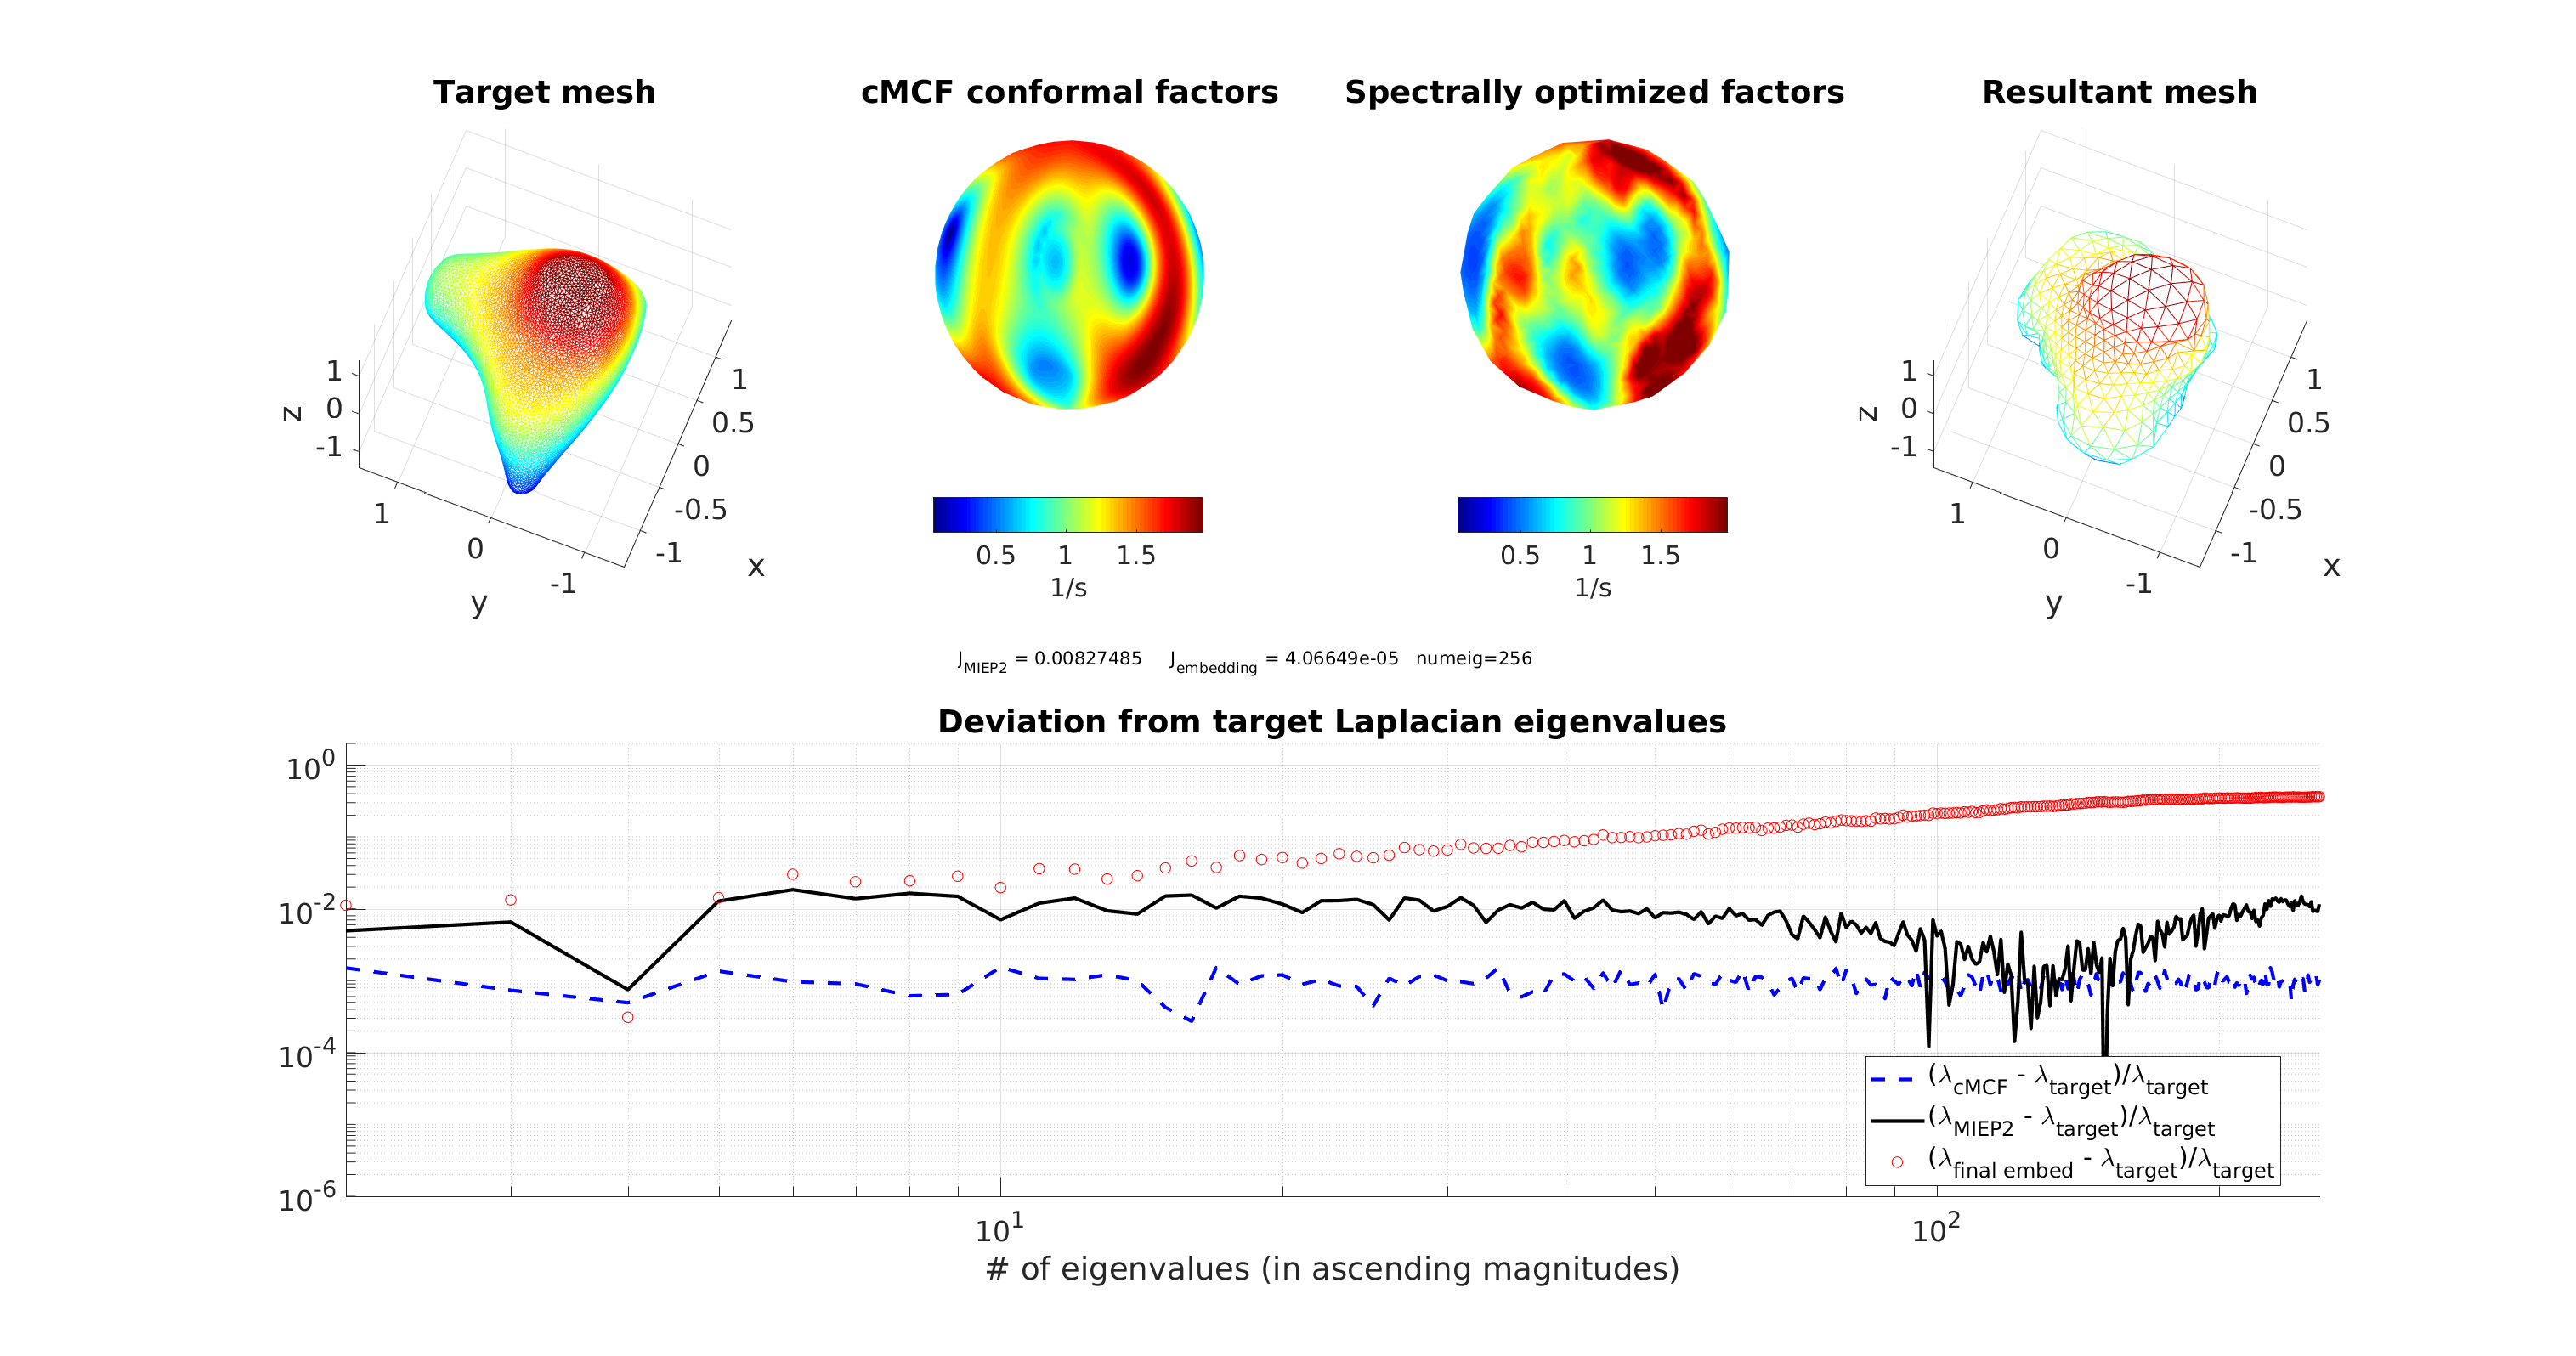
\includegraphics[width=1.2\textwidth]{{{eps/i2_540_t3_blob18k_a256e256L30}}}
	\caption{a=256, L=30x30}
\end{figure}

\subsubsection{regularized}

\begin{figure}[H]
	\hspace*{-6em}
	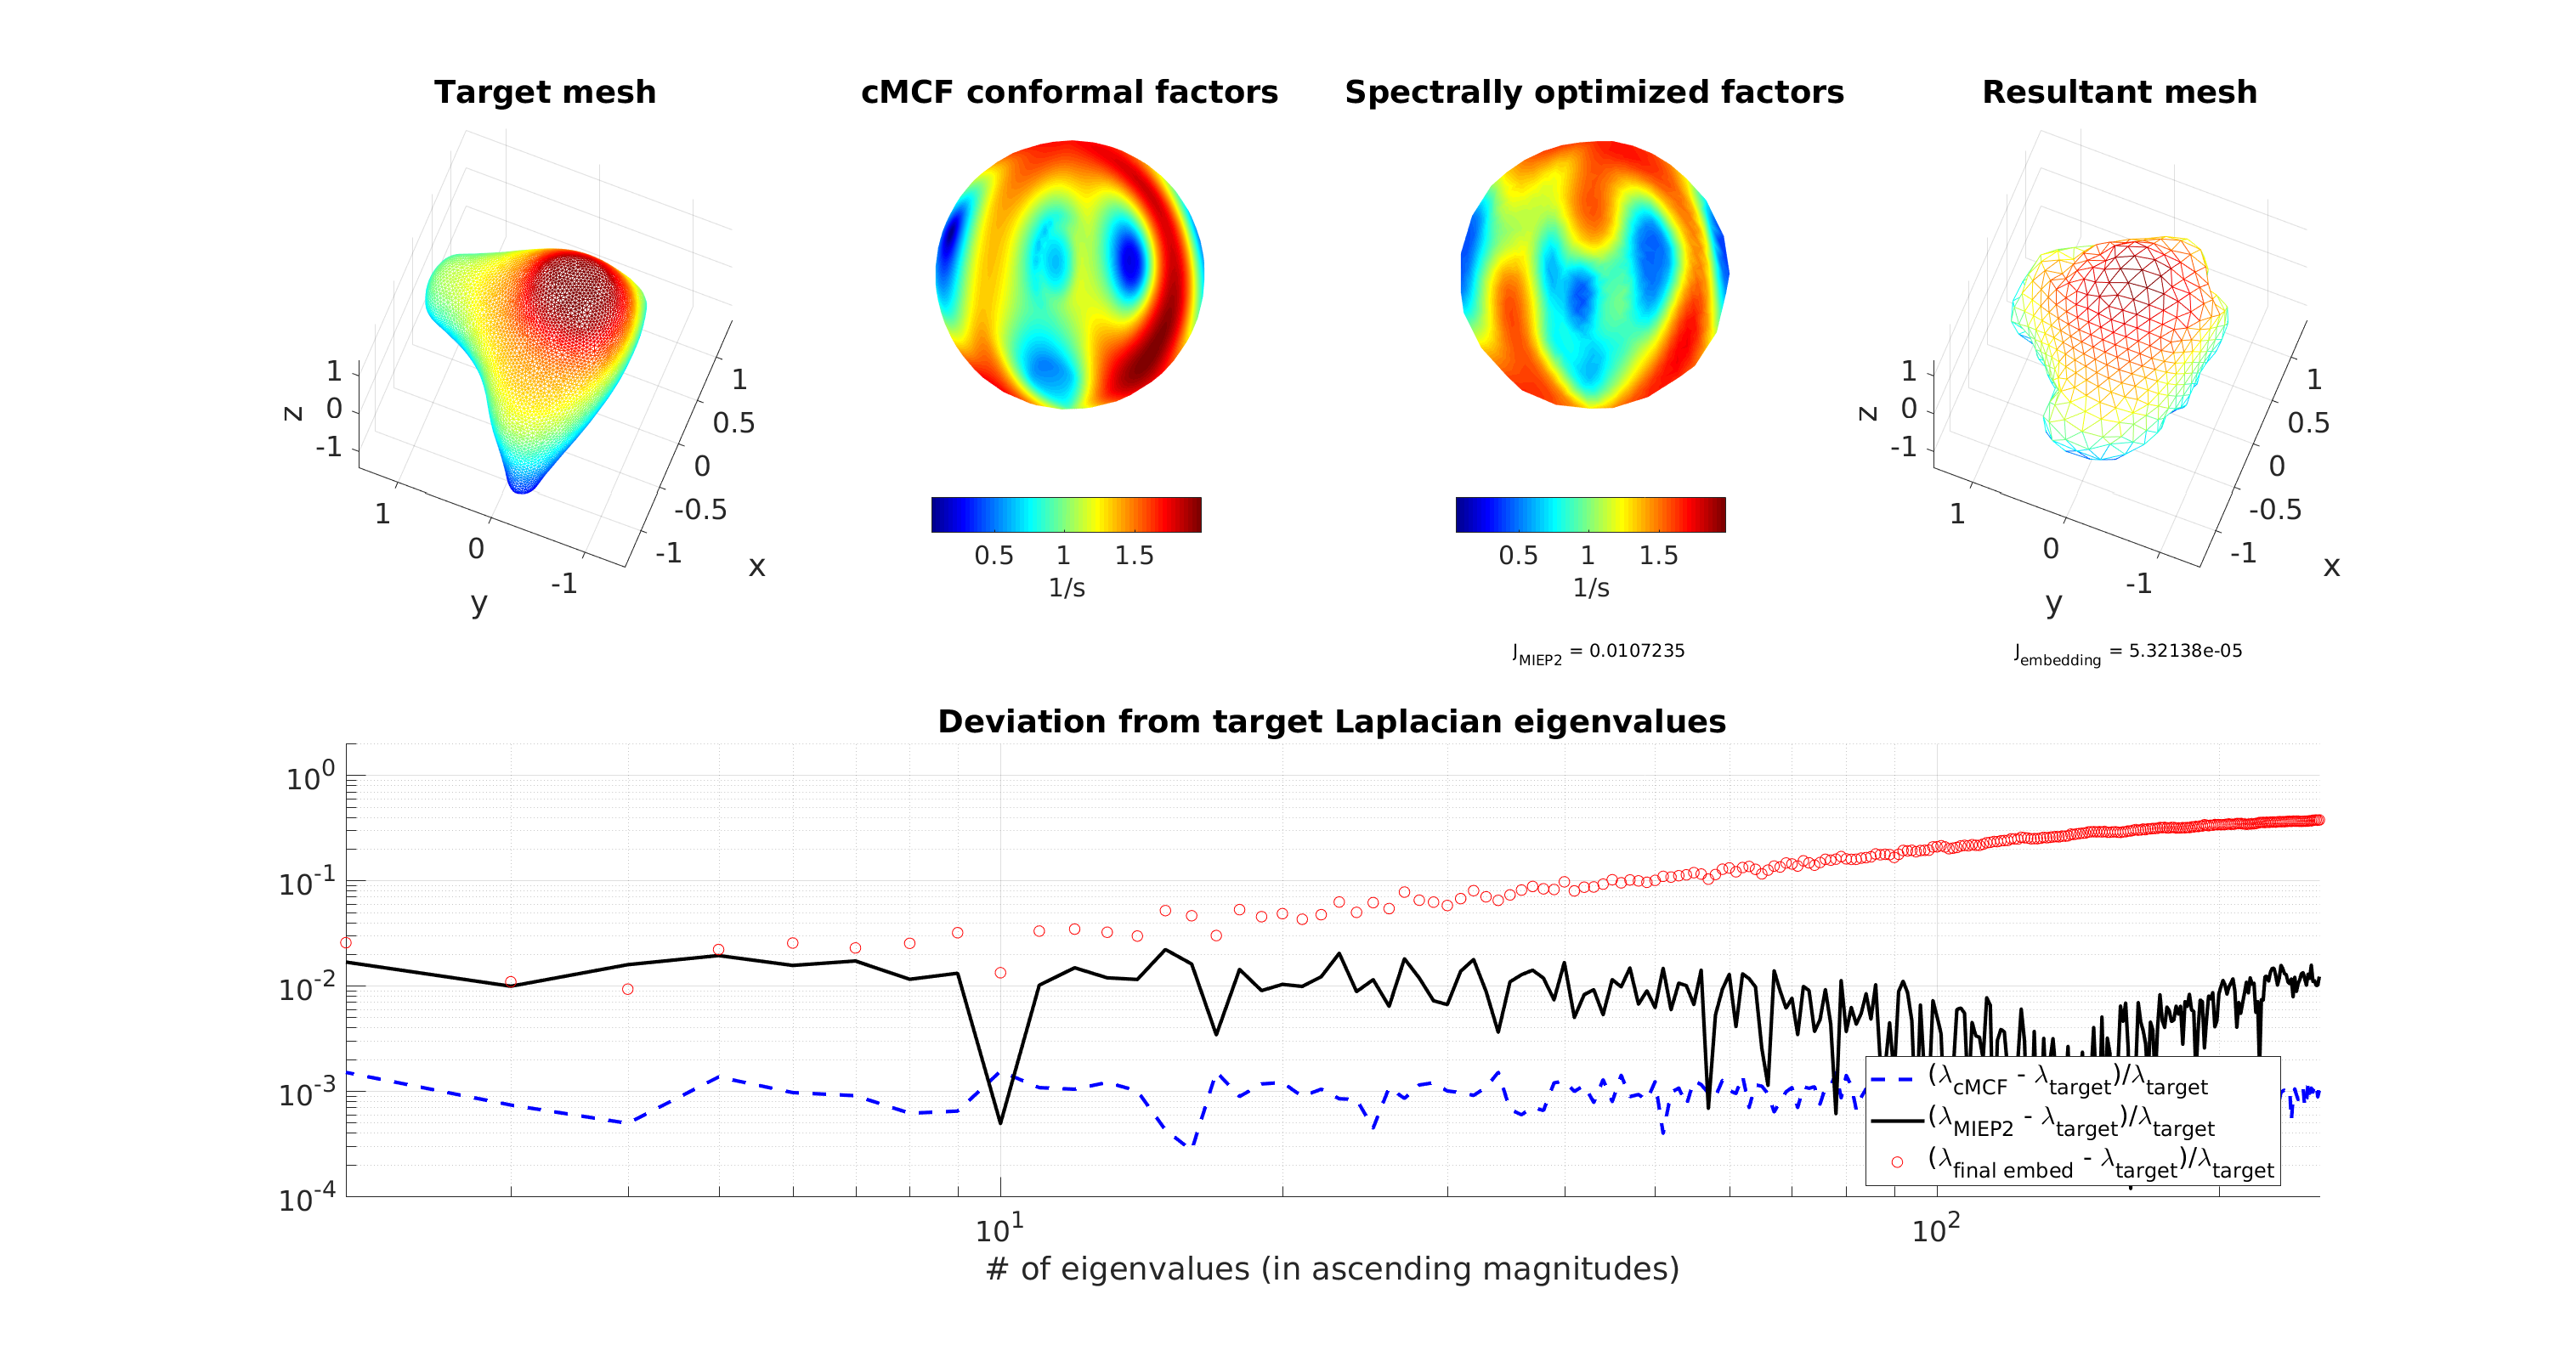
\includegraphics[width=1.2\textwidth]{{{eps/i2_540_t3_blob18k_a256e256L30r1e-06}}}
	\caption{a=256, L=30x30, R=1e-6}
\end{figure}

\section{A To-Do list}
\subsection{M\"obius balancing routine}
For reference, Prof.~Keenan Crane have a write-up and working C codes in his geometry processing toolset. The current MATLAB implementation is experiencing (too much?) oscillatory behavior possibly due to some sort of silly bug.

%\subsection{Regularization in spherical harmonics basis}
%if we make an equivalence between low-high frequency to spherical harmonic basis coefficients, we can assume (the analogy is from conditions on function being smooth and its Fourier coefficients) the coefficients must decrease as much as possible as soon as possible for the smoothiest solution.
%Naively, we can add a term $\propto \sum_i w_i a_{l,m}^2$ to the cost where $w_i$ grows at the appropriate rate (e.g. $exp(l)$ or $l^k$ for some positive $k>1$). But this did not work so well.

\subsection{Structured optimization}
Again assuming the above equivalence, it might stand to reason that we shall first optimize for lower frequency features ($a_{l,m}$ with small $l$?) and then move on to refining the higher frequency ones.

Related to this is that there is no indication how many coefficient should be used.

\subsection{Precomputing more 3j symbols}
maybe it will be worthwhile to utilize some state-of-the-art method to calculate as many 3j symbols as one's RAM can handle to eliminate this uncertainty for the experiments.

Reference: 
\url{http://epubs.siam.org/doi/abs/10.1137/S1064827503422932}

\subsection{Topology}
We also would like to calculate the topology of the surface from the spectrum beforehand. In the smooth setting, we can infer these from the \textbf{asymptotics} of heat trace from the spectrum. In the discrete case, it is not immediate how to extract these information. A reference is found to mention successfully doing this through some sort of curve fitting. Or is this a suitable task for machine learning? And after knowing a topology with $g\geq1$, can be also use the corresponding harmonic basis functions?

Reference: Martin Reuter, Franz-Erich Wolter, Niklas Peinecke, ``Laplace-Beltrami spectra as `Shape-DNA' of surfaces and solids''

\url{http://reuter.mit.edu/blue/papers/reuter-shapeDNA06/reuter-shapeDNA06.pdf}

\subsection{Adaptive remeshing for the simplical inverse problem}
Since it works pretty well in the simplicial setting when we regularize and use enough eigenvalues (up to embedding issues), the only obstacle barring us from full victory is the apparent need to assume MCF starting mesh. The idea to improve here is to remesh at each step according to the current conformal factor solution. Practically speaking, it might preserve more sanity to try these in a better development environment (so no more MATLAB non OOP shenanigans, at least not with the built-in BFGS optimization algorithm).

\subsection{Embedding problem}
Visually and numerically, it seems that we can obtain spectrally optimized conformal factors that matches the desired cMCF ones. However, the (again) na\"ive way of re-inflating a sphere using a scalar conformal factor field seems to less than efficient, as in we need very fine meshes and the na\"ive algorithm scales with number of meshes used squared. But this should be a problem that others have and will continue to tackle even on their own.
\end{document}